\chapter{الأنظمة العابرة: الرتبة الأولى والرتبة الثانية}\label{ch:b1:transient-regimes}

اضغط على زاوية سيارة واقفة ثم اترْكها. فالسيارة السليمة
ترتفع مرة واحدة وتتوقف؛ أما السيارة ذات المخمّدات البالية فترتجّ مرتين أو
ثلاثًا قبل أن تستقرّ. وفي مختبر إلكترونيات يظهر السلوكان نفسهما
على راسم الاهتزاز حين يتفرّغ مكثف عبر
وشيعة: عودة سلسة، أو رنين يخبو. وكلاهما
\emph{عابر} بين حالة مستقرة وأخرى، وكلاهما يخضع
لعائلة صغيرة واحدة من المعادلات التفاضلية الخطية --- الرتبة الأولى
لمخزن طاقة واحد، والرتبة الثانية لمخزنين يتبادلان. ويحلّ هذا
الفصل هذه المعادلات مرة واحدة وإلى الأبد، ويسمّي وسائطها (\omterm{def:b1:transient-regimes:firstorder}{ثابت
الزمن}، \omterm{def:b1:transient-regimes:secondorder}{والتواتر الزاوي الذاتي}، \omterm{def:b1:transient-regimes:secondorder}{وعامل الجودة})، ويبيّن كيف تصف الأعداد
نفسها دارةً كهربائية ونظامَ تعليق.

\begin{omfigure}
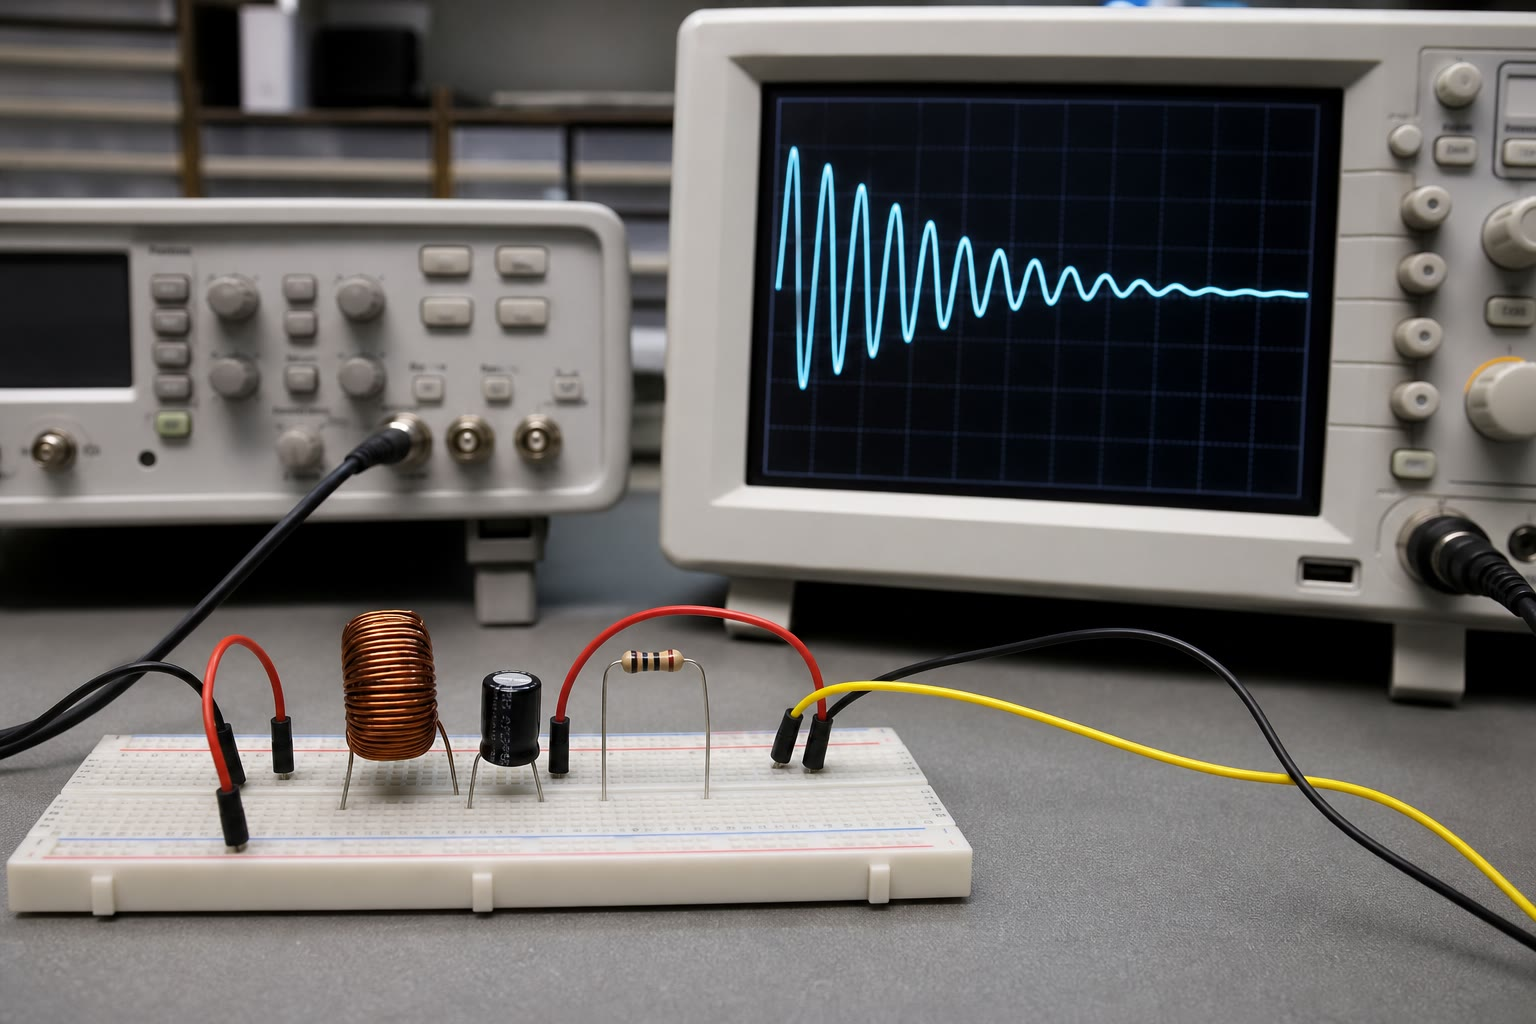
\includegraphics[width=0.60\linewidth]{images/book3/ai/b3-07-rlc-breadboard-oscilloscope.jpg}

{\small وشيعة ومكثف \omterm{def:b1:dc-circuits:resistor}{وناقلة أومية} على لوحة تجارب، وعلى راسم الاهتزاز التذبذب المتناقص الذي يعقب قفزة: وهو \omterm{thm:b1:transient-regimes:regimes}{النظام شبه الدوري} في هذا الفصل.}
\end{omfigure}

\section{أنظمة الرتبة الأولى}

\begin{definition}[الجملة الخطية من الرتبة الأولى]\label{def:b1:transient-regimes:firstorder}
\index{جملة من الرتبة الأولى}\index{ثابت الزمن}\index{نظام عابر}\index{نظام دائم}
يحقق مقدار $x(t)$ \emph{معادلة خطية من الرتبة الأولى ذات
معاملات ثابتة} حين يكون
\[
\tau\,\frac{\dd x}{\dd t} + x = x_\infty ,
\]
حيث $\tau > 0$ هو \emph{ثابت الزمن} و $x_\infty$ ثابت (وهو
القيمة التي يفرضها المنبع). و\emph{نظامه الدائم} هو $x = x_\infty$؛
و\emph{النظام العابر} هو الاقتراب منه انطلاقًا من القيمة
الابتدائية $x(0) = x_0$.
\end{definition}

\begin{theorem}[الحلّ]\label{thm:b1:transient-regimes:firstorder}
الحلّ الوحيد الذي يحقق $x(0) = x_0$ هو
\[
x(t) = x_\infty + (x_0 - x_\infty)\,\eu^{-t/\tau} .
\]
وتتقلّص الفجوة إلى \omterm{def:b1:transient-regimes:firstorder}{النظام الدائم} بالعامل $\eu^{-1} \approx
0.37$ في كل $\tau$: أي $63\%$ من الطريق عند $\tau$، و$95\%$ عند $3\tau$،
و$99\%$ عند $4.6\tau$. والمماس عند المبدأ يبلغ $x_\infty$ عند
$t = \tau$.
\end{theorem}

\begin{proof}
المقدار $y = x - x_\infty$ يحقق $\tau y' + y = 0$، وحلوله
$y = K\eu^{-t/\tau}$ (ويبرهن درس الرياضيات في المعادلات التفاضلية
الخطية على أنه لا حلول غيرها)؛ ومنه $K = x_0 - x_\infty$. والميل
عند $0$ هو $-(x_0 - x_\infty)/\tau$، وهو ما كان سيغلق الفجوة في الزمن
$\tau$.
\end{proof}

\begin{omfigure}
\begin{tikzpicture}
\begin{axis}[omaxis, width=9.4cm, height=5.4cm, xlabel={$t$}, ylabel={$x$},
    xmin=0, xmax=5, ymin=0, ymax=1.35, xtick={1,2,3,4,5},
    xticklabels={$\tau$,$2\tau$,$3\tau$,$4\tau$,$5\tau$},
    ytick={0.632,1}, yticklabels={$0.63$,$x_\infty$}]
  \addplot[omExo, dashed, domain=0:5, samples=2] {1};
  \addplot[omExo, dashed, domain=0:1, samples=2] {x};
  \addplot[omDef, thick, domain=0:5, samples=100] {1 - exp(-x)};
  \draw[dashed, omExo] (axis cs:1,0) -- (axis cs:1,0.632) -- (axis cs:0,0.632);
  \draw[dashed, omExo] (axis cs:3,0) -- (axis cs:3,0.95);
  \node[omExo, below right, font=\footnotesize] at (axis cs:3,0.95) {$0.95\,x_\infty$};
  \node[omDef, font=\footnotesize, below right] at (axis cs:2.2,0.75) {$x_\infty(1 - \eu^{-t/\tau})$};
\end{axis}
\end{tikzpicture}

{\small استجابة الرتبة الأولى لقفزة انطلاقًا من $x_0 = 0$: يلاقي المماس
الابتدائي المقاربَ عند $t = \tau$؛ و$63\%$ من الطريق عند $\tau$،
و$95\%$ عند $3\tau$. وكل عابر من الرتبة الأولى هو هذا المنحني، ممطوطًا
بمقدار $\tau$ ومنزاحًا بمقدار $x_0$ و $x_\infty$.}
\end{omfigure}

\begin{proposition}[الدارتان RC و RL]\label{prop:b1:transient-regimes:rcrl}
\index{دارة RC}\index{دارة RL}
مكثف $C$ يُشحن عبر \omterm{def:b1:dc-circuits:resistor}{ناقلة أومية} $R$ من منبع مثالي $E$
يحقق $RC\,\dd u_C/\dd t + u_C = E$: أي $\tau = RC$ و $u_{C,\infty} = E$. و
وشيعة $L$ على التسلسل مع $R$ تحت $E$ تحقق $(L/R)\,\dd i/\dd t + i =
E/R$: أي $\tau = L/R$ و $i_\infty = E/R$. وبنزع المنبع
($E \to 0$) تصف المعادلتان نفساهما التفريغ نحو الصفر.
\end{proposition}

\begin{proof}
قانون الحلقات $E = Ri + u_C$ مع $i = C\,\dd u_C/\dd t$؛ وقانون الحلقات
$E = Ri + L\,\dd i/\dd t$.
\end{proof}

\begin{proposition}[شرطا الاتصال]\label{prop:b1:transient-regimes:continuity}
\index{اتصال $u_C$ و $i_L$}
التوتر بين طرفَي مكثف والتيار في وشيعة دالتان
متصلتان بالزمن: فعند لحظة قطع $t_0$ يكون
$u_C(t_0^+) = u_C(t_0^-)$ و $i_L(t_0^+) = i_L(t_0^-)$. أما التيارات في
الناقلات الأومية والتوترات بين طرفَي الوشائع فقد تقفز.
\end{proposition}

\begin{proof}
قفزة في $u_C$ كانت ستقتضي $i = C\,\dd u_C/\dd t$ لانهائيًّا، وقفزة
في $i_L$ كانت ستقتضي $u = L\,\dd i/\dd t$ لانهائيًّا؛ وكلاهما
مستحيل في دارة توتراتها وتياراتها منتهية (أو على نحو مكافئ،
لا تستطيع الطاقتان المخزونتان $\tfrac12 Cu_C^2$ و $\tfrac12 Li^2$ أن تتغيرا
لحظيًّا دون استطاعة لانهائية).
\end{proof}

\begin{method}[حلّ عابر من الرتبة الأولى]\label{met:b1:transient-regimes:first}
\begin{enumerate}
  \item اكتب قانونَي الحلقات والعقد بعد القاطع، مع
        قوانين العناصر؛ واختزل إلى معادلة واحدة في $u_C$ أو $i_L$ و
        ضعها على الصورة $\tau x' + x = x_\infty$؛ ثم اقرأ $\tau$ و
        $x_\infty$ (وهذا الأخير هو أيضًا \omterm{def:b1:transient-regimes:firstorder}{النظام الدائم} الذي يُوجد
        باستبدال دارة مفتوحة بالمكثف $C$ وسلك بالوشيعة $L$).
  \item أوجد $x_0$ من اتصال $u_C$ أو $i_L$ عبر
        لحظة القطع، مستعملًا الدارة \emph{قبلها}.
  \item اكتب $x = x_\infty + (x_0 - x_\infty)\eu^{-t/\tau}$؛ ثم استنتج
        المقادير الأخرى بالاشتقاق وبقانون الحلقات.
\end{enumerate}
وحين يرى المكثف شبكة من الناقلات والمنابع، تُستبدل
بتلك الشبكة مكافئُ تيفنان $(E_{\mathrm{Th}}, R_{\mathrm{Th}})$
أولًا (\cref{ch:b1:dc-circuits}): فيكون $\tau = R_{\mathrm{Th}}C$ و
$u_\infty = E_{\mathrm{Th}}$.
\end{method}

\begin{proposition}[الحصيلة الطاقية لشحن RC]\label{prop:b1:transient-regimes:rcenergy}
عند شحن مكثف من $0$ إلى $E$ عبر أيّ \omterm{def:b1:dc-circuits:resistor}{ناقلة أومية} $R$، يقدّم
المنبع $CE^2$، ويخزّن المكثف $\tfrac12 CE^2$، وتبدد
الناقلة النصف الآخر $\tfrac12 CE^2$ --- مهما تكن $R$.
\end{proposition}

\begin{proof}
لدينا $i = (E/R)\eu^{-t/\tau}$؛ ويقدّم المنبع $\int_0^\infty Ei\,\dd t
= E \cdot (E/R)\tau = CE^2$؛ وتأخذ الناقلة $\int_0^\infty Ri^2\,\dd t
= (E^2/R)\int_0^\infty \eu^{-2t/\tau}\dd t = (E^2/R)(\tau/2) = \tfrac12 CE^2$؛
والفرق هو المخزون $\tfrac12 CE^2$. وقيمة أصغر للمقاومة $R$ تبدد
الطاقة نفسها أسرع.
\end{proof}

\begin{example}[وشيعة مرحّل]\label{ex:b1:transient-regimes:relay}
$L = \qty{20}{mH}$ و $R = \qty{5.0}{\ohm}$ و $E = \qty{10}{V}$: فيكون $\tau =
\qty{4.0}{ms}$ و $i_\infty = \qty{2.0}{A}$؛ وتنجذب الملامسات حين
يبلغ $i$ مقدار \qty{1.5}{A}، أي عند $t = -\tau\ln(1 - 0.75) =
\qty{5.5}{ms}$. وعند فتح الدارة يجب أن يهبط $i$ من \qty{2}{A}؛ و
ثنائي ``الدوران الحرّ'' الموضوع على طرفَي الوشيعة يمنحه مسارًا عبر $R$
وحدها، فيكون $\tau = \qty{4}{ms}$ بدلًا من شرارة.
\end{example}

\section{أنظمة الرتبة الثانية}

\begin{definition}[الصورة النظامية للرتبة الثانية]\label{def:b1:transient-regimes:secondorder}
\index{جملة من الرتبة الثانية}\index{تواتر زاوي ذاتي}\index{عامل الجودة}\index{نسبة التخميد}
يكون المقدار $x(t)$ \emph{جملةً خطية من الرتبة الثانية} حين يكون
\[
\frac{\dd^2 x}{\dd t^2} + \frac{\omega_0}{Q}\,\frac{\dd x}{\dd t} + \omega_0^2\,x
= \omega_0^2\,x_\infty ,
\]
حيث $\omega_0 > 0$ هو \emph{\omterm{def:b1:wave-propagation:signal}{التواتر الزاوي} الذاتي}، و $Q > 0$ هو
\emph{عامل الجودة} (وهو عديم البعد)، و $x_\infty$ هو \omterm{def:b1:transient-regimes:firstorder}{النظام الدائم}.
ويُكتب أيضًا $\omega_0/Q = 2\xi\omega_0$ حيث $\xi = 1/2Q$ هي
\emph{نسبة التخميد}.
\end{definition}

\begin{proposition}[الدارة RLC على التسلسل]\label{prop:b1:transient-regimes:rlc}
\index{دارة RLC}
مكثف $C$ ووشيعة $L$ \omterm{def:b1:dc-circuits:resistor}{وناقلة أومية} $R$ على التسلسل تحت منبع
$E$: يحقق توتر المكثف الصورةَ النظامية مع
\[
\omega_0 = \frac{1}{\sqrt{LC}}, \qquad Q = \frac{1}{R}\sqrt{\frac{L}{C}},
\qquad u_{C,\infty} = E .
\]
\end{proposition}

\begin{proof}
قانون الحلقات: $E = L\,\dd i/\dd t + Ri + u_C$ مع $i = C\,\dd u_C/\dd t$:
ومنه $LC\,u_C'' + RC\,u_C' + u_C = E$؛ ثم نقسم على $LC$ ونطابق
$\omega_0^2 = 1/LC$ و $\omega_0/Q = R/L$.
\end{proof}

\begin{omfigure}
\begin{tikzpicture}[font=\small]
  \draw (0,0) to[battery1, l=$E$, invert] (0,2.6) to[R=$R$] (2.4,2.6) to[L=$L$, i=$i$] (4.8,2.6) -- (4.8,2.6) to[C=$C$, v=$u_C$] (4.8,0) -- (0,0);
  \begin{scope}[xshift=7.6cm]
    \draw[thick] (0,0) -- (0,3.4);
    \fill[pattern=north east lines] (-0.25,0) rectangle (0,3.4);
    % spring
    \draw[thick] (0,2.6) -- (0.4,2.6) \foreach \i in {0,...,5} {-- ++(0.2,0.25) -- ++(0.2,-0.5) -- ++(0.2,0.25)} -- (3.3,2.6);
    % damper
    \draw[thick] (0,0.8) -- (1.2,0.8);
    \draw[thick] (1.2,0.5) -- (1.2,1.1) -- (2.2,1.1); \draw[thick] (1.2,0.5) -- (2.2,0.5);
    \draw[thick] (1.9,0.6) -- (1.9,1.0); \draw[thick] (1.9,0.8) -- (3.3,0.8);
    \draw[thick, fill=omDef!15] (3.3,0.2) rectangle (4.5,3.2); \node at (3.9,1.7) {$m$};
    \draw[-Stealth] (3.9,3.5) -- (5.2,3.5) node[right] {$x$};
    \node at (1.7,3.15) {$k$}; \node at (1.7,0.1) {$\alpha$};
  \end{scope}
\end{tikzpicture}

{\small الوجهان الاثنان \omterm{def:b1:transient-regimes:secondorder}{للجملة من الرتبة الثانية}: \omterm{prop:b1:transient-regimes:rlc}{الدارة RLC}
على التسلسل ($\omega_0 = 1/\sqrt{LC}$ و $Q = \sqrt{L/C}/R$) وجملة
الكتلة--النابض--المخمّد ($\omega_0 = \sqrt{k/m}$ و $Q = \sqrt{km}/\alpha$).
معادلة واحدة وأنظمة ثلاثة هي نفسها.}
\end{omfigure}

\begin{proposition}[المتذبذب الميكانيكي]\label{prop:b1:transient-regimes:mechanical}
\index{الكتلة--النابض--المخمّد}\index{تناظر كهرميكانيكي}
كتلة $m$ على نابض صلابته $k$ مع مخمّد لزج
معامله $\alpha$ (والقوة $-\alpha\dot x$)، منزاحة بمقدار $x$ عن
التوازن، تحقق $m\ddot x + \alpha\dot x + kx = 0$: أي الصورة النظامية
مع
\[
\omega_0 = \sqrt{\frac{k}{m}}, \qquad Q = \frac{\sqrt{km}}{\alpha} .
\]
والتقابل $x \leftrightarrow q$ و $\dot x \leftrightarrow i$ و
$m \leftrightarrow L$ و $\alpha \leftrightarrow R$ و $k \leftrightarrow 1/C$
ينقل كل نتيجة من إحدى الجملتين إلى الأخرى.
\end{proposition}

\begin{proof}
قانون نيوتن الثاني (\cref{ch:b1:newton-dynamics}) مع قوة النابض
$-kx$ وقوة التخميد؛ ثم نقسم على $m$.
\end{proof}

\begin{theorem}[الأنظمة الثلاثة]\label{thm:b1:transient-regimes:regimes}
\index{نظام لا دوري}\index{نظام حرج}\index{نظام شبه دوري}\index{شبه الدور}
تُحكَم حلول المعادلة المتجانسة $x'' + (\omega_0/Q)x' +
\omega_0^2 x = 0$ بجذور المعادلة $r^2 + (\omega_0/Q)r +
\omega_0^2 = 0$، ذات المميّز $\Delta = \omega_0^2(1/Q^2 - 4)$:
\begin{itemize}
  \item من أجل $Q < \tfrac12$، \emph{النظام اللادوري}: جذران حقيقيان سالبان
        $r_\pm = -\frac{\omega_0}{2Q}\big(1 \mp \sqrt{1 - 4Q^2}\big)$، و
        $x = A\eu^{r_+t} + B\eu^{r_-t}$، أي عودة بلا تذبذب؛
  \item من أجل $Q = \tfrac12$، \emph{\omterm{thm:b1:transient-regimes:regimes}{النظام الحرج}}: جذر مضاعف $r = -\omega_0$، و
        $x = (A + Bt)\eu^{-\omega_0 t}$، أي أسرع عودة دون
        تجاوز؛
  \item من أجل $Q > \tfrac12$، \emph{\omterm{thm:b1:transient-regimes:regimes}{النظام شبه الدوري}}: جذران عقديان
        $r = -1/\tau \pm \iu\omega$ مع
        \[
        \tau = \frac{2Q}{\omega_0}, \qquad
        \omega = \omega_0\sqrt{1 - \frac{1}{4Q^2}},
        \qquad
        x = \eu^{-t/\tau}\big(A\cos\omega t + B\sin\omega t\big),
        \]
        أي تذبذب مخمَّد \emph{شبه دوره} $T = 2\pi/\omega$
        داخل الغلاف $\pm\sqrt{A^2 + B^2}\,\eu^{-t/\tau}$.
\end{itemize}
والحلّ الكامل مع طرف أيمن ثابت هو $x_\infty$ زائد
الحلّ المتجانس؛ ويُوجد $A$ و $B$ من $x(0)$ و $x'(0)$.
\end{theorem}

\begin{proof}
المعادلة المميِّزة لمعادلة خطية ذات معاملات
ثابتة (درس الرياضيات، المعادلات الخطية من الرتبة الثانية):
جذراها $r = -\omega_0/2Q \pm \tfrac12\sqrt\Delta$. ومن أجل $Q > \tfrac12$ يكون
$\sqrt\Delta = \iu\omega_0\sqrt{4 - 1/Q^2}$، فيعطي الجزء الحقيقي
$-\omega_0/2Q = -1/\tau$ والجزء التخيلي $\pm\omega_0\sqrt{1 - 1/4Q^2}$؛
والحلول الحقيقية هي تراكيب $\eu^{-t/\tau}\cos\omega t$
و $\eu^{-t/\tau}\sin\omega t$.
\end{proof}

\begin{omfigure}
\begin{tikzpicture}
\begin{axis}[omaxis, width=11.5cm, height=6cm, xlabel={$\omega_0 t$}, ylabel={$x/x_\infty$},
    xmin=0, xmax=16, ymin=0, ymax=1.75, xtick={0,5,10,15}, ytick={0.5,1,1.5},
    legend style={at={(0.97,0.97)}, anchor=north east, font=\footnotesize, draw=none, fill=none}]
  % Q=0.2: roots r = -(1/(2Q))(1 -/+ sqrt(1-4Q^2)) = -2.5(1 -/+ 0.6) = -1, -4 ; x = 1 - (4 e^{-t} - e^{-4t})/3
  \addplot[omProp, thick, domain=0:16, samples=200] {1 - (4*exp(-x) - exp(-4*x))/3};
  \addlegendentry{$Q = 0.2$ (لا دوري)}
  \addplot[omThm, thick, domain=0:16, samples=200] {1 - (1 + x)*exp(-x)};
  \addlegendentry{$Q = 0.5$ (حرج)}
  % Q=3: tau=6, w = sqrt(1-1/36)=0.986 ; x = 1 - e^{-t/6}(cos wt + sin wt /(6 w))
  \addplot[omDef, thick, domain=0:16, samples=400] {1 - exp(-x/6)*(cos(deg(0.986*x)) + sin(deg(0.986*x))/(6*0.986))};
  \addlegendentry{$Q = 3$ (شبه دوري)}
  \addplot[omExo, dashed, domain=0:16, samples=2] {1};
\end{axis}
\end{tikzpicture}

{\small استجابة \omterm{def:b1:transient-regimes:secondorder}{جملة من الرتبة الثانية} لقفزة انطلاقًا من السكون، من أجل ثلاثة
عوامل جودة. فمع $Q$ صغير: زحف بطيء؛ ومع $Q = \tfrac12$: أسرع
عودة دون تجاوز؛ ومع $Q$ كبير: رنين يدوم نحو $Q$
تذبذبة.}
\end{omfigure}

\begin{proposition}[قراءة $Q$ على أثر شبه دوري]\label{prop:b1:transient-regimes:decrement}
\index{تناقص لوغاريتمي}
في \omterm{thm:b1:transient-regimes:regimes}{النظام شبه الدوري} تكون نسبة قيمتين عظميين متتاليتين
$x_{n+1}/x_n = \eu^{-T/\tau}$؛ و\emph{\omterm{prop:b1:transient-regimes:decrement}{التناقص اللوغاريتمي}}
\[
\delta = \ln\frac{x_n}{x_{n+1}} = \frac{T}{\tau} = \frac{\pi}{Q\sqrt{1 - 1/4Q^2}}
\approx \frac{\pi}{Q} \quad (Q \gg 1)
\]
يعطي $Q$؛ وعدد التذبذبات المرئية قبل أن تهبط السعة
دون $5\%$ هو نحو $Q$. ومن أجل $Q \gg 1$ يكون $\omega \approx \omega_0$
و $T \approx 2\pi/\omega_0$.
\end{proposition}

\begin{proof}
الغلاف $\eu^{-t/\tau}$ يُضرب في $\eu^{-T/\tau}$ في كل دور؛
و$T/\tau = (2\pi/\omega)(\omega_0/2Q)$. والغلاف يبلغ $\eu^{-3}
\approx 5\%$ عند $3\tau = 6Q/\omega_0 \approx Q\,T$، أي بعد نحو
$Q$ دورًا.
\end{proof}

\begin{omfigure}
\begin{tikzpicture}
\begin{axis}[omaxis, width=11.5cm, height=5.6cm, xlabel={$t$}, ylabel={$x$},
    xmin=0, xmax=12.5, ymin=-1.2, ymax=1.3, xtick={2,4,6,8,10,12},
    xticklabels={$T$,$2T$,$3T$,$4T$,$5T$,$6T$}, ytick={-1,1}, yticklabels={$-x_0$,$x_0$}]
  \addplot[omExo, dashed, domain=0:12.5, samples=60] {exp(-x/5)};
  \addplot[omExo, dashed, domain=0:12.5, samples=60] {-exp(-x/5)};
  \addplot[omDef, thick, domain=0:12.5, samples=500] {exp(-x/5)*cos(deg(pi*x))};
  \fill[omThm] (axis cs:0,1) circle (1.4pt) node[above right, font=\footnotesize] {$x_0$};
  \fill[omThm] (axis cs:2,0.670) circle (1.4pt) node[above right, xshift=2pt, yshift=3pt, font=\footnotesize] {$x_1 = x_0\eu^{-T/\tau}$};
  \fill[omThm] (axis cs:4,0.449) circle (1.4pt) node[above right, xshift=2pt, yshift=3pt, font=\footnotesize] {$x_2$};
\end{axis}
\end{tikzpicture}

{\small تناقص حرّ شبه دوري، $x = x_0\eu^{-t/\tau}\cos\omega t$:
تتقلّص القيم العظمى المتتالية بالعامل الثابت $\eu^{-T/\tau}$، و
$\ln(x_n/x_{n+1}) = T/\tau \approx \pi/Q$ يقيس \omterm{def:b1:transient-regimes:secondorder}{عامل الجودة}
من الأثر.}
\end{omfigure}

\begin{example}[رنين دارة RLC]\label{ex:b1:transient-regimes:rlcnum}
$L = \qty{10}{mH}$ و $C = \qty{100}{nF}$ و $R = \qty{100}{\ohm}$:
فيكون $\omega_0 = 1/\sqrt{10^{-9}} = \qty{3.16e4}{rad/s}$ (أي $f_0 =
\qty{5.03}{kHz}$)، و $Q = \sqrt{L/C}/R = 316/100 = 3.16$: \omterm{thm:b1:transient-regimes:regimes}{فالنظام شبه دوري}،
و $\tau = 2Q/\omega_0 = \qty{0.20}{ms}$، و $\omega = 0.987\,\omega_0$، و
$T = \qty{0.20}{ms}$، وثلاث تذبذبات مرئية. والمقاومة الحرجة
هي $R_c = 2\sqrt{L/C} = \qty{632}{\ohm}$؛ وفوقها يكون التفريغ
لا دوري.
\end{example}

\begin{method}[حلّ عابر من الرتبة الثانية]\label{met:b1:transient-regimes:second}
\begin{enumerate}
  \item اكتب المعادلة؛ وضعها على الصورة النظامية؛ ثم اقرأ $\omega_0$
        و $Q$ و $x_\infty$.
  \item حدّد النظام من $Q$ واكتب الحلّ العام
        $x_\infty$ زائد الحلّ المتجانس.
  \item أوجد $x(0)$ و $x'(0)$ من اتصال $u_C$ و $i_L$
        (وفي \omterm{prop:b1:transient-regimes:rlc}{الدارة RLC}: $u_C(0^+) = u_C(0^-)$ و $u_C'(0^+) = i(0^-)/C$)؛
        ثم حلّ لإيجاد الثابتين.
\end{enumerate}
\end{method}

\begin{example}[الشروط الابتدائية]\label{ex:b1:transient-regimes:ic}
المكثف في المثال السابق مشحون إلى $U_0$، وعند
$t = 0$ يُغلَق على $L$ و $R$ (بلا منبع): فيكون $x_\infty = 0$ و
$u_C(0) = U_0$ و $u_C'(0) = i(0)/C = 0$ لأن تيار الوشيعة كان معدومًا.
ومنه $A = U_0$ و $-A/\tau + B\omega = 0$ و $B = U_0/(\omega\tau) =
U_0/\sqrt{4Q^2 - 1}$: أي $u_C = U_0\eu^{-t/\tau}[\cos\omega t + \sin(\omega
t)/\sqrt{4Q^2 - 1}]$ --- ومن أجل $Q \gg 1$ يصير ببساطة $U_0\eu^{-t/\tau}\cos\omega_0 t$،
ويبلغ التيار $i = -C\,\dd u_C/\dd t$ ذروته قرب $U_0\sqrt{C/L} =
U_0/(\omega_0 L)$.
\end{example}

\begin{remark}[الطاقة]\label{rem:b1:transient-regimes:energy}
الطاقة المخزونة $\tfrac12 Cu_C^2 + \tfrac12 Li^2$ (أو $\tfrac12 kx^2
+ \tfrac12 m\dot x^2$) تتناقص بالمعدل $Ri^2$ (أو $\alpha\dot x^2$):
بالاشتقاق واستعمال المعادلة. وفي كل شبه دور تتقلّص الطاقة
بالعامل $\eu^{-2T/\tau}$؛ ومع $Q = 3$ يضيع نحو $88\%$ منها
في كل تذبذبة. و$Q$ العالي يعني تسربًا بطيئًا نسبةً إلى
التذبذب --- أي ساعة جيدة، ورنينًا حادًّا
(\cref{ch:b1:sinusoidal-impedance}) --- و$Q$ المنخفض يعني عودة سريعة:
وهو الخيار الصحيح لنظام تعليق أو لإبرة مقياس.
\end{remark}

\section{تمارين}

\begin{exercise}[$\star$]\label{exo:b1:transient-regimes:1}
\omterm{prop:b1:transient-regimes:rcrl}{دارة RC}: $R = \qty{10}{k\ohm}$ و $C = \qty{47}{nF}$، تُشحن من
$E$. احسب $\tau$ و $u_C(\tau)/E$ والزمن اللازم لبلوغ $99\%$ من $E$.
\end{exercise}

\begin{exercise}[$\star$]\label{exo:b1:transient-regimes:2}
\omterm{prop:b1:transient-regimes:rcrl}{دارة RL}: $L = \qty{20}{mH}$ و $R = \qty{5.0}{\ohm}$ و $E = \qty{10}{V}$.
احسب $\tau$ والتيار النهائي والتيار عند $t = \tau$ و
التوتر بين طرفَي الوشيعة بُعيد إغلاق القاطع.
\end{exercise}

\begin{exercise}[$\star$]\label{exo:b1:transient-regimes:3}
\omterm{prop:b1:transient-regimes:rlc}{دارة RLC} على التسلسل: $L = \qty{10}{mH}$ و $C = \qty{100}{nF}$ و $R = \qty{100}{\ohm}$.
احسب $\omega_0$ و $f_0$ و $Q$؛ وسمِّ النظام؛ وأعطِ $\tau$ و
\omterm{thm:b1:transient-regimes:regimes}{شبه الدور}.
\end{exercise}

\begin{exercise}[$\star$]\label{exo:b1:transient-regimes:4}
من أجل $L$ و $C$ نفسيهما، أيّ مقاومة تعطي \omterm{thm:b1:transient-regimes:regimes}{النظام الحرج}؟
وما $Q$ عندئذٍ؟ وماذا يحدث من أجل $R = \qty{2}{k\ohm}$؟
\end{exercise}

\begin{exercise}[$\star\star$]\label{exo:b1:transient-regimes:5}
مكثف مشحون $C = \qty{1.0}{\micro F}$ يتفرّغ عبر ناقلة
مجهولة $R$؛ ويتنصّف التوتر كل \qty{3.5}{ms}. بيّن أن
زمن التنصّف هو $\tau\ln 2$ وأوجد $R$.
\end{exercise}

\begin{exercise}[$\star\star$]\label{exo:b1:transient-regimes:6}
بيّن بالمكاملة المباشرة أن شحن مكثف من $0$ إلى $E$
عبر $R$ يبدد بالضبط مقدار $\tfrac12 CE^2$ في $R$، مستقلًّا عن
$R$. وماذا يصير مردود النقل، وكيف يمكن
تحسينه؟
\end{exercise}

\begin{exercise}[$\star\star$]\label{exo:b1:transient-regimes:7}
على راسم اهتزاز يُظهر تناقص RLC حرّ قيمًا عظمى متتالية قدرها
\qty{2.0}{V} و\qty{1.5}{V} و\qty{1.12}{V} بفواصل قدرها \qty{0.40}{ms}.
استنتج $Q$ و $\omega_0$، ثم، مع $C = \qty{1.0}{\micro F}$، قيمتَي
$L$ و $R$.
\end{exercise}

\begin{exercise}[$\star\star$]\label{exo:b1:transient-regimes:8}
مكثف مشحون إلى $U_0 = \qty{100}{V}$ (حيث $C = \qty{10}{\micro F}$)
يُوصل إلى وشيعة $L = \qty{1.0}{mH}$ مقاومتها صغيرة ($Q \gg 1$).
اكتب $u_C(t)$ و $i(t)$، وقدّر التيار الأعظمي. وأين تقع
الطاقة عند الذروة؟
\end{exercise}

\begin{exercise}[$\star\star$]\label{exo:b1:transient-regimes:9}
ربع سيارة: $m = \qty{400}{kg}$ على نابض $k = \qty{2.0e4}{N/m}$.
احسب $\omega_0$ و $f_0$ ومعامل التخميد الحرج. ومع
مخمّد $\alpha = \qty{2000}{N.s/m}$، أعطِ $Q$ والنظام و
\omterm{thm:b1:transient-regimes:regimes}{شبه الدور} وزمن التناقص $\tau$.
\end{exercise}

\begin{exercise}[$\star\star\star$]\label{exo:b1:transient-regimes:10}
وشيعة $L = \qty{0.50}{H}$ تحمل $I_0 = \qty{2.0}{A}$؛ ثم يُفصل المنبع
وتُترك الوشيعة على ناقلة تصريف $R = \qty{100}{\ohm}$.
أعطِ $i(t)$ و $\tau$ والتوتر الأعظمي بين طرفَي الوشيعة والطاقة
المتبددة. وماذا كان سيحدث بلا الناقلة؟
\end{exercise}

\begin{exercise}[$\star\star\star$]\label{exo:b1:transient-regimes:11}
مكثف $C = \qty{1.0}{\micro F}$ يُشحن من $E = \qty{12}{V}$
عبر $R_1 = \qty{10}{k\ohm}$ بينما تكون $R_2 = \qty{20}{k\ohm}$ موصولة
على طرفيه. باستعمال مكافئ تيفنان، أوجد \omterm{def:b1:transient-regimes:firstorder}{ثابت الزمن} و
التوتر النهائي؛ واكتب $u_C(t)$ انطلاقًا من $u_C(0) = 0$.
\end{exercise}

\begin{exercise}[$\star\star\star$]\label{exo:b1:transient-regimes:12}
\omterm{thm:b1:transient-regimes:regimes}{النظام الحرج}، قفزة من السكون ($x(0) = x'(0) = 0$): بيّن أن
$x = x_\infty[1 - (1 + \omega_0 t)\eu^{-\omega_0 t}]$، وأوجد
عدديًّا الزمن اللازم لبلوغ $95\%$ من $x_\infty$ (بوحدة
$1/\omega_0$). وقارنه بزمن استقرار الغلاف من أجل $Q = 5$
ومن أجل الجذر البطيء حين $Q = 0.1$؛ واستنتج لماذا يكون ``الحرج'' هو
هدف المهندس.
\end{exercise}

\section{مسألة: تصميم نظام تعليق}

\begin{problem}[{مسألة نهاية الأسبوع --- المعادلة التفاضلية نفسها على
طاولة تجارب وتحت سيارة: كم ارتجاجة يسمح بها مخمّد بالٍ،
وماذا يختار المصمّم بدلًا من ذلك، وكيف يميّز عدد واحد
بين الحالتين}]
\label{pb:b1:transient-regimes:1}
يدرس الجزء I \omterm{prop:b1:transient-regimes:rlc}{دارة RLC} على التسلسل، $L = \qty{10}{mH}$ و $C = \qty{100}{nF}$؛
وتدرس الأجزاء من II إلى IV نموذج ربع سيارة: كتلة $m = \qty{350}{kg}$ ترتكز على
نابض $k = \qty{22}{kN/m}$ ومخمّد صدمات يؤثر بالقوة $-\alpha\dot x$.
وتجاوز استجابة القفزة في \omterm{thm:b1:transient-regimes:regimes}{النظام شبه الدوري} (معطى):
$x_{\max}/x_\infty - 1 = \exp(-\pi\xi/\sqrt{1 - \xi^2})$، مع $\xi = 1/2Q$.

\medskip
\noindent\textbf{الجزء I --- الدارة.}
\begin{enumerate}
  \item اكتب قانون الحلقات \omterm{prop:b1:transient-regimes:rlc}{للدارة RLC} على التسلسل تحت منبع $E$، ثم
        المعادلة التفاضلية التي يحققها $u_C$.
  \item ضعها على الصورة النظامية؛ وعبّر عن $\omega_0$ و $Q$.
  \item احسب $\omega_0$ و $f_0$ والمقاومة الحرجة $R_c$.
  \item اكتب المعادلة المميِّزة ومميّزها؛ واذكر
        الأنظمة الثلاثة بدلالة $Q$.
  \item في الحالة شبه الدورية، أعطِ $\tau$ و $\omega$ و
        صورة $u_C(t)$.
  \item من أجل $R = \qty{100}{\ohm}$ احسب $Q$ و $\tau$ \omterm{thm:b1:transient-regimes:regimes}{وشبه الدور}،
        وعدد التذبذبات المرئية.
  \item المكثف، وقد شُحن إلى $U_0$، يُوصل إلى $L$ و $R$
        عند $t = 0$. أعطِ $u_C(0^+)$ و $\dd u_C/\dd t(0^+)$، مع
        السبب الفيزيائي لكلٍّ منهما.
\end{enumerate}

\medskip
\noindent\textbf{الجزء II --- ربع السيارة.}
\begin{enumerate}[resume]
  \item بقياس $x$ من وضع التوازن، اكتب قانون نيوتن
        الثاني للهيكل وبيّن أن الوزن يسقط من المعادلة.
  \item ضع المعادلة على الصورة النظامية؛ وأعطِ $\omega_0$ و $Q$ بدلالة
        $m$ و $k$ و $\alpha$، واذكر التقابلات
        الكهرميكانيكية.
  \item احسب $\omega_0$ و $f_0$ والمعامل الحرج
        $\alpha_c$.
  \item يركّب المصمّم $\alpha = \qty{4000}{N.s/m}$: احسب $Q$ و
        $\xi$، وسمِّ النظام.
  \item احسب $\tau$ \omterm{thm:b1:transient-regimes:regimes}{وشبه الدور}.
  \item احسب التجاوز بعد قفزة (كرصيف): فهل السيارة
        مريحة؟
  \item أيّ مقاومة $R$ تعطي دارة الجزء I عاملَ الجودة $Q$
        نفسه الذي لنظام التعليق هذا؟
\end{enumerate}

\medskip
\noindent\textbf{الجزء III --- المخمّد البالي.}
تسرّب الزيت: $\alpha = \qty{1200}{N.s/m}$.
\begin{enumerate}[resume]
  \item احسب $Q$ \omterm{thm:b1:transient-regimes:regimes}{وشبه الدور} و $\tau$.
  \item بأيّ عامل تتقلّص القيم العظمى المتتالية؟ وكم ارتجاجة
        تُرى قبل أن تهبط السعة دون $5\%$؟
  \item اختبار الارتجاج: يُضغط ركن السيارة إلى الأسفل بمقدار $x_0 =
        \qty{5.0}{cm}$ ثم يُترك. أعطِ الشروط الابتدائية و
        الطاقة المخزونة في النابض، وقل أين تذهب تلك الطاقة.
  \item قدّر السرعة العظمى للهيكل خلال العودة
        الأولى ($\approx x_0\omega_0$ من أجل $Q \gg 1$) والقوة العظمى
        في المخمّد.
  \item لماذا لا يكون التخميد الحرج تمامًا ($Q = \tfrac12$) خيار
        المصمّم، مع أنه لا يعطي أيّ تجاوز؟ (فكّر في
        المليمترات الأخيرة من العودة.)
  \item احسب التجاوز من أجل المخمّد البالي وقارنه بما
        وجدته في الجزء II.
\end{enumerate}

\medskip
\noindent\textbf{الجزء IV --- تشخيص $Q$ من أثر.}
يسجّل مقياس تسارع على الهيكل التناقص الحرّ.
\begin{enumerate}[resume]
  \item من أجل السيارة البالية تقرأ القيم العظمى المتتالية $1.00$ و$0.25$ و$0.062$
        (بوحدات اعتباطية). احسب \omterm{prop:b1:transient-regimes:decrement}{التناقص اللوغاريتمي}، واستنتج
        $\xi$ بالضبط من $\delta = 2\pi\xi/\sqrt{1 - \xi^2}$، ثم $Q$؛
        وقارن بالجزء III.
  \item ومن أجل السيارة السليمة لا تُرى قيمة عظمى ثانية؛ ولا يمكن قراءة إلا
        التجاوز، $3.8\%$. اقلب صيغة التجاوز لإيجاد
        $\xi$ و $Q$.
  \item أيّ كسر من الطاقة الميكانيكية يبدده المخمّد البالي
        في كل شبه دور؟
  \item فنّيّ لا سيارة لديه يبني \omterm{prop:b1:transient-regimes:rlc}{الدارة RLC} في الجزء I
        مع $R$ مختارة بحيث $Q = 2.3$: فما $R$، ولماذا يكون أثر
        راسم الاهتزاز، مرسومًا بدلالة $\omega_0 t$، مطابقًا في
        الشكل لأثر السيارة؟
  \item لخّص: أيّ عدد عديم البعد يقرّر شكل أيّ
        عابر من الرتبة الثانية، وأيّ قيمة يستهدفها مصمّم نظام التعليق،
        وماذا ينبغي أن يستنتج السائق من ``أكثر من ارتجاجة
        واحدة''.
\end{enumerate}
\end{problem}
